\section{Executable Expert Organizations}\label{sec:organization}
\subsection{Representation and execution}
An organization revision is
\begin{equation}
\mathcal O_v=(R_v,G_v,P_v,K_v,A_v,F_v;\,h_v).
\label{eq:organization}
\end{equation}
$R_v$ is the set of expert roles. $G_v$ is a collection of directed acyclic graphs whose nodes name roles and whose edges declare task-level dependencies. $P_v$ contains the orchestrator and expert instructions. $K_v$ contains model-readable skills, procedures, references, and examples. $A_v$ maps the orchestrator and roles to declared capability references, including tools and skills. $F_v$ is the complete package file set, containing these resources and any executable or opaque assets. The content digest $h_v$ identifies the exact revision; a human-readable version label is additional metadata.

A role may occur in different workflow declarations, so roles and workflow nodes are distinct objects. The graphs expose intended dependencies to the orchestrator. Dispatch remains an LLM decision using predecessor evidence, active workers, and execution capacity; graph validity is not a proof that every dependency is semantically satisfied at runtime.

For task $x$, execution produces a trajectory $\tau$ and deliverable $y$:
\begin{equation}
(\tau,y)\sim \operatorname{Run}_{\phi}
   (\mathcal O_v,x,\eta,b).
\label{eq:run}
\end{equation}
Here $\phi$ fixes the foundation model and inference configuration, $\eta$ specifies the workspace, tools, permissions, and external environment, and $b$ is the task budget. The task stores an immutable package binding. Worker descriptors carry the corresponding projected capabilities and revision identity. Conversation state, intermediate artifacts, and scheduler ownership belong to the execution, rather than to the reusable organization.

Figure~\ref{fig:organization} shows the representation through the Research Studio package. Its five expert roles cover planning, research, analysis, fact checking, and writing. The analyst produces canonical computation evidence before fact checking; the writer renders the accepted evidence rather than recomputing numerical claims. These are declared responsibilities and workflow relationships in the inspected package \citep{ocsource}.

The same package declares three workflows with different entry conditions. Full research uses all five roles when the assignment requires new source collection. Evidence synthesis starts with the analyst when a sufficient source bundle is already supplied. Direct writing uses the writer alone for bounded material that requires faithful presentation without new research claims. These alternatives reuse the same role definitions and resources; they do not require a separately maintained organization for each task shape. Choosing among them remains part of the orchestrator's task interpretation. A task with missing computational evidence cannot become a direct-writing task merely by asking the writer to supply the missing calculations.

\begin{figure}[!t]
\centering
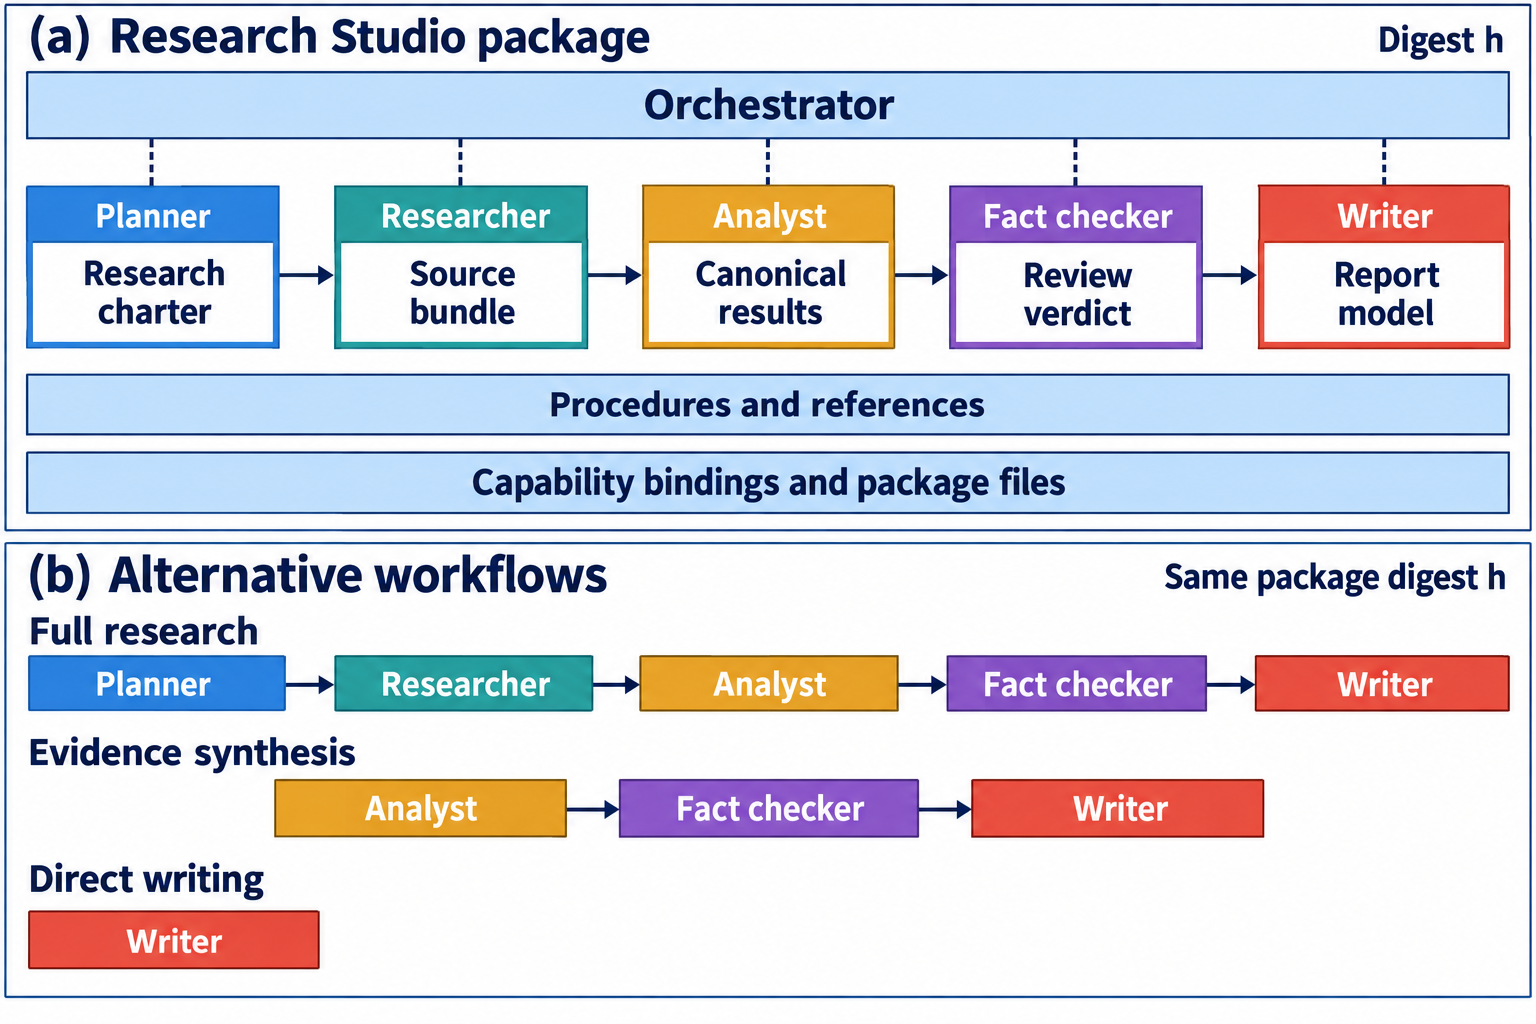
\includegraphics[width=\linewidth]{figures/architecture.png}
\caption{A reusable organization and its task-specific workflow choices. The five expert roles, their output types, and the three alternative workflow declarations follow Research Studio. The image abbreviates the package digest $h_v$ as $h$. Solid role-to-role arrows are declared dependencies; dashed orchestrator links indicate LLM dispatch. The resource bands belong to the package, while outputs and execution state belong to individual tasks.}
\label{fig:organization}
\end{figure}


\subsection{Domain specialization}
We express a domain specification as $\mathcal D=(\mathcal X,K^{\mathcal D},A^{\mathcal D},C^{\mathcal D},q^{\mathcal D})$: a task family, domain procedures, required capabilities, output contracts, and an evaluation rubric. A specialization operation
\begin{equation}
\mathcal O^{\mathcal D}_0
  =\operatorname{Specialize}(\mathcal O_{\mathrm{base}},\mathcal D)
\label{eq:specialization}
\end{equation}
constructs a package with explicit role responsibilities and resource bindings. $C^{\mathcal D}$ and $q^{\mathcal D}$ are analytical names for the domain's artifact schemas, checking procedures, and scorers; they are not additional mandatory manifest fields.

For evidence-based analysis, specialization assigns collection and citation procedures to the researcher, executable calculations and canonical result schemas to the analyst, verification criteria to the fact checker, and a report template to the writer. The evaluation checks numerical agreement with the canonical results, claim support, and delivery requirements. Replacing the names with professional titles while keeping tools, procedures, and acceptance criteria unchanged is an insufficient specialization.

Initial specialization can introduce domain resources and authorized tools. Subsequent evolution operates within the parent package's inherited capability envelope and frozen executable resources. This separates establishing what an organization can access from learning how it uses those resources. It also makes the comparison with a fixed specialized organization meaningful: both start with the same professional substrate.


\subsection{A concrete professional contract}\label{sec:contract}
The analytical-report specialization gives organizational knowledge three connected forms. A \emph{procedure} explains how to perform a recurring operation, such as reconciling a source population before aggregating it. A \emph{resource binding} makes the corresponding input, tool, schema, or reference available to the responsible role. An \emph{artifact contract} describes the evidence a downstream role needs before using the output. These forms have different failure modes: good instructions cannot compensate for an unavailable source, and an available calculation tool does not specify which population or units are appropriate.

For a report task, the planner fixes the question, source hierarchy, comparison dimensions, and stopping conditions. The researcher assembles durable sources and identifies disagreement. The analyst records the calculation method, source identities, canonical tables, and claim-to-result correspondence. The fact checker examines those post-computation claims and records corrections and unresolved limits. The writer constructs a structured report model from the accepted material and derives its presentation from that model. This allocation follows the Research Studio instructions \citep{ocsource}. It places the numerical method upstream of verification and presentation, so a persuasive final report is not the only object available for inspection.

To make the handoff precise, consider a quantitative claim $\kappa$. Its analytical support record can be written as $(\kappa,r,a,\ell_{\mathrm{rev}})$, where $r$ identifies a canonical result revision, $a$ locates the relevant table cell or range, and $\ell_{\mathrm{rev}}$ identifies the review addressing that claim and result. This notation describes the information relationship, not a new mandatory runtime schema. A complete record still needs semantic checking: the table may use the wrong population, the cited range may not entail the prose, or the review may leave the claim unresolved. The writer's contract therefore concerns both locating the resources and preserving the accepted meaning, units, qualifications, and uncertainty.

The reusable package contains the rules for constructing and checking such relationships. Task-specific sources, computed values, and accepted conclusions remain in the task's evidence. Thus, specializing an organization for analytical reporting does not require installing the answer to each report in its prompts. It establishes a procedure that can be applied to different questions, source bundles, and result tables. Whether this procedure transfers well is measured on new tasks with separately constructed evidence.
